\documentclass{standalone}
\usepackage{tikz}
\usepackage{ctex,siunitx,bm}
\setCJKmainfont{Noto Serif CJK SC}
\usepackage{tkz-euclide,ninecolors}
\usepackage{amsmath}
\usetikzlibrary{patterns, calc}
\usetikzlibrary {decorations.pathmorphing, decorations.pathreplacing, decorations.shapes,}
\begin{document}
\small
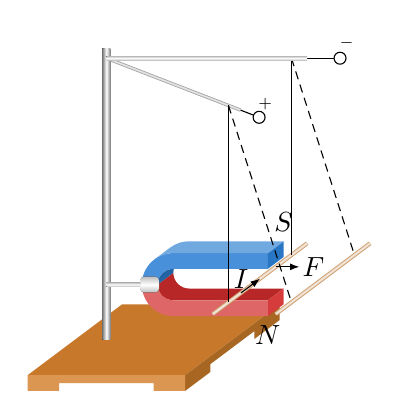
\begin{tikzpicture}[>=latex,yscale=1.0]
  \fill[brown6](-1.85,-1.15)--(0.15,-1.15)--(1.35,-0.25)--(-0.65,-0.25)--cycle;
  \fill[brown5]( 0.15,-1.35)--( 0.47,-1.11)--( 0.47,-1.01)--( 1.03,-0.59)--( 1.03,-0.69)--( 1.35,-0.45)--( 1.35,-0.25)--( 0.15,-1.15)--cycle;
  \fill[brown7]( 0.15,-1.15)--( 0.15,-1.35)--(-0.25,-1.35)--(-0.25,-1.25)--(-1.45,-1.25)--(-1.45,-1.35)--(-1.85,-1.35)--(-1.85,-1.15)--cycle;
  \fill[left color=gray, right color=gray,middle color=white](-0.9,-0.7)rectangle(-0.8,3);
  \fill[red4](-0.2,0)arc(180:270:0.2)--++(1.2,0)--++(0.2,0.15)--++(-1.2,0)arc(270:180:0.2)--cycle;
  \fill[red5](1.2,-0.2)--++(0.2,0.15)--++(0,-0.2)--++(-0.2,-0.15)--cycle;
  \fill[red6](-0.4,0)arc(180:270:0.4)--++(1.2,0)node[below,text=black]{$N$}--++(0,0.2)--++(-1.2,0)arc(270:180:0.2)--cycle;
  \foreach \w in {80.60,40,20}
  {
    \draw[line width={1.5*sin(\w)},brown!\w](0.5,-0.375)--(1.7,0.525);
    \draw[line width={1.5*sin(\w)},brown!\w](1.3,-0.375)--(2.5,0.525);
    \draw[line width={1.2*sin(\w)},gray!\w](-0.85,2.875)--(0.855,2.215);
  }
  \draw[arrows={-Latex[scale=0.7]},thin](0.86,-0.105)--(1.1,0.075)node[at start,above,inner sep=1.5pt]{$I$};
  \draw[arrows={-Latex[scale=0.7]},thin](1.3,0.225)--++(0.3,0)node[right,inner sep=1pt]{$F$};
  \fill[azure4](-0.2,0)arc(180:90:0.2)--++(0.2,0.15)arc(90:180:0.2)--cycle;
  \fill[azure6](-0.4,0)arc(180:90:0.4)--++(1.2,0)--++(0,-0.2)--++(-1.2,0)arc(90:180:0.2)--cycle;
  \fill[azure5](1.2,0.4)--++(0.2,0.15)node[above,text=black]{$S$}--++(0,-0.2)--++(-0.2,-0.15)--cycle;
  \fill[azure7](1.2,0.4)--++(0.2,0.15)--++(-1.2,0)arc(90:126.87:0.4)--++(-0.2,-0.15)arc(126.87:90:0.4)--cycle;
  \draw(0.7,-0.225)--++(0,2.5)(1.5,0.375)--++(0,2.5);
  \draw[densely dashed](0.7,2.275)--(1.5,-0.225)(1.5,2.875)--(2.3,0.375);
  \draw[-o](0.855,2.215)--(1.1663,2.0945)node[above]{\tiny$+$};
  \draw[-o](1.7,2.875)--++(0.5,0)node[above]{\tiny$-$};
  \fill[top color=lightgray,bottom color=lightgray,middle color=white](-0.85,2.9)rectangle(1.7,2.85);
  \fill[top color=lightgray,bottom color=lightgray,middle color=white,rounded corners=0.5mm](-0.42,-0.1)rectangle(-0.18,0.1);
  \fill[top color=lightgray,bottom color=lightgray,middle color=white](-0.85,-0.025)rectangle(-0.42,0.025);
\end{tikzpicture}
\end{document}